\documentclass[conference]{IEEEtran}
\usepackage[utf8]{inputenc}
\usepackage{graphicx}
\usepackage{amsmath}
\usepackage{cite}
\usepackage{float}

\title{Clasificaci\'on de Im\'agenes Histopatol\'ogicas de C\'ancer de Pulm\'on Usando Redes Neuronales Convolucionales Residuales}

\author{\IEEEauthorblockN{Joel Ibaceta}
\IEEEauthorblockA{\textit{Universidad Nacional de Ingenieria} \\
joel.ibaceta.c@uni.pe}}

\begin{document}

\maketitle

\begin{abstract}
Este estudio presenta un modelo basado en redes neuronales convolucionales residuales para la clasificación automática de imágenes histopatológicas de cáncer de pulmón. Utilizando el conjunto de datos LC25000, se entrena una red personalizada tipo ResNet-18, denominada \textit{ResNetLung}, diseñada desde cero para distinguir entre tres tipos de tejido pulmonar: adenocarcinoma, carcinoma de células escamosas y tejido sano. El modelo alcanza una precisión final del 95.61 \% sobre el conjunto de validación, mostrando un comportamiento robusto y generalizable. Los resultados respaldan el potencial de estas arquitecturas para asistir en el diagnóstico médico automatizado basado en imágenes.
\end{abstract}

\section{Introducci\'on}

El cáncer de pulmón es una de las principales causas de mortalidad a nivel mundial. El diagnóstico temprano mediante análisis histopatológico es esencial para mejorar el pronóstico, pero requiere tiempo, recursos especializados y experiencia médica considerable. La automatización de esta tarea mediante técnicas de inteligencia artificial puede acelerar y estandarizar la detección de patrones patológicos.

En este trabajo, se propone un modelo convolucional residual, denominado \textit{ResNetLung}, implementado desde cero con una arquitectura tipo ResNet-18. El modelo es entrenado para clasificar imágenes histológicas teñidas con hematoxilina y eosina en tres categorías clínicas relevantes: tejido pulmonar sano, adenocarcinoma y carcinoma de células escamosas. Se reporta un rendimiento superior al 95 \% en tareas de validación, lo que sugiere su aplicabilidad en entornos clínicos asistidos por computadora.

\section{Metodolog\'ia}

\section{Dataset}

Se utilizó el conjunto de datos LC25000, del cual se seleccionaron únicamente las clases relacionadas al pulmón: adenocarcinoma (\texttt{lung\_aca}), tejido sano (\texttt{lung\_n}) y carcinoma de células escamosas (\texttt{lung\_scc}). Cada clase contiene imágenes histopatológicas teñidas con hematoxilina y eosina (H\&E), capturadas con aumentos microscópicos homogéneos.

La Figura~\ref{fig:dataset} muestra una selección de imágenes representativas para cada clase, donde se pueden observar diferencias visuales en la morfología celular y la estructura del tejido.

\begin{figure}[H]
\centering
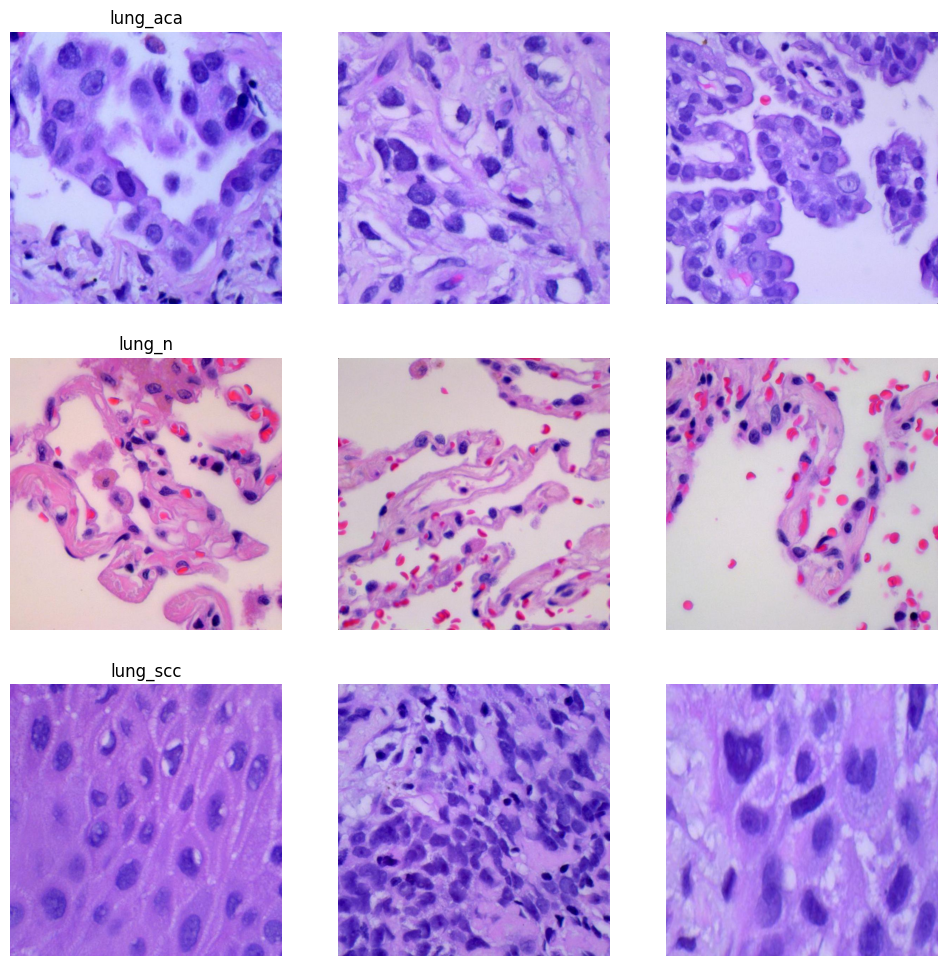
\includegraphics[width=0.48\textwidth]{dataset_exploration.png}
\caption{Ejemplos de imágenes histopatológicas por clase: adenocarcinoma (arriba), tejido sano (medio), y carcinoma escamoso (abajo).}
\label{fig:dataset}
\end{figure}

\subsection{Arquitectura del Modelo}

Se implementa una arquitectura tipo ResNet, denominada \textit{ResNetLung}, con una configuración equivalente a ResNet-18. Esta red está compuesta por: una capa convolucional inicial, cuatro bloques residuales con [2,2,2,2] bloques cada uno, una capa de \textit{pooling} global y una capa densa final. Esto da lugar a un total de 18 capas entrenables.

La Figura~\ref{fig:architecture} ilustra visualmente la arquitectura propuesta, destacando el flujo de datos a través de las capas convolucionales y residuales, así como la operación final de clasificación.

\begin{figure}[H]
\centering
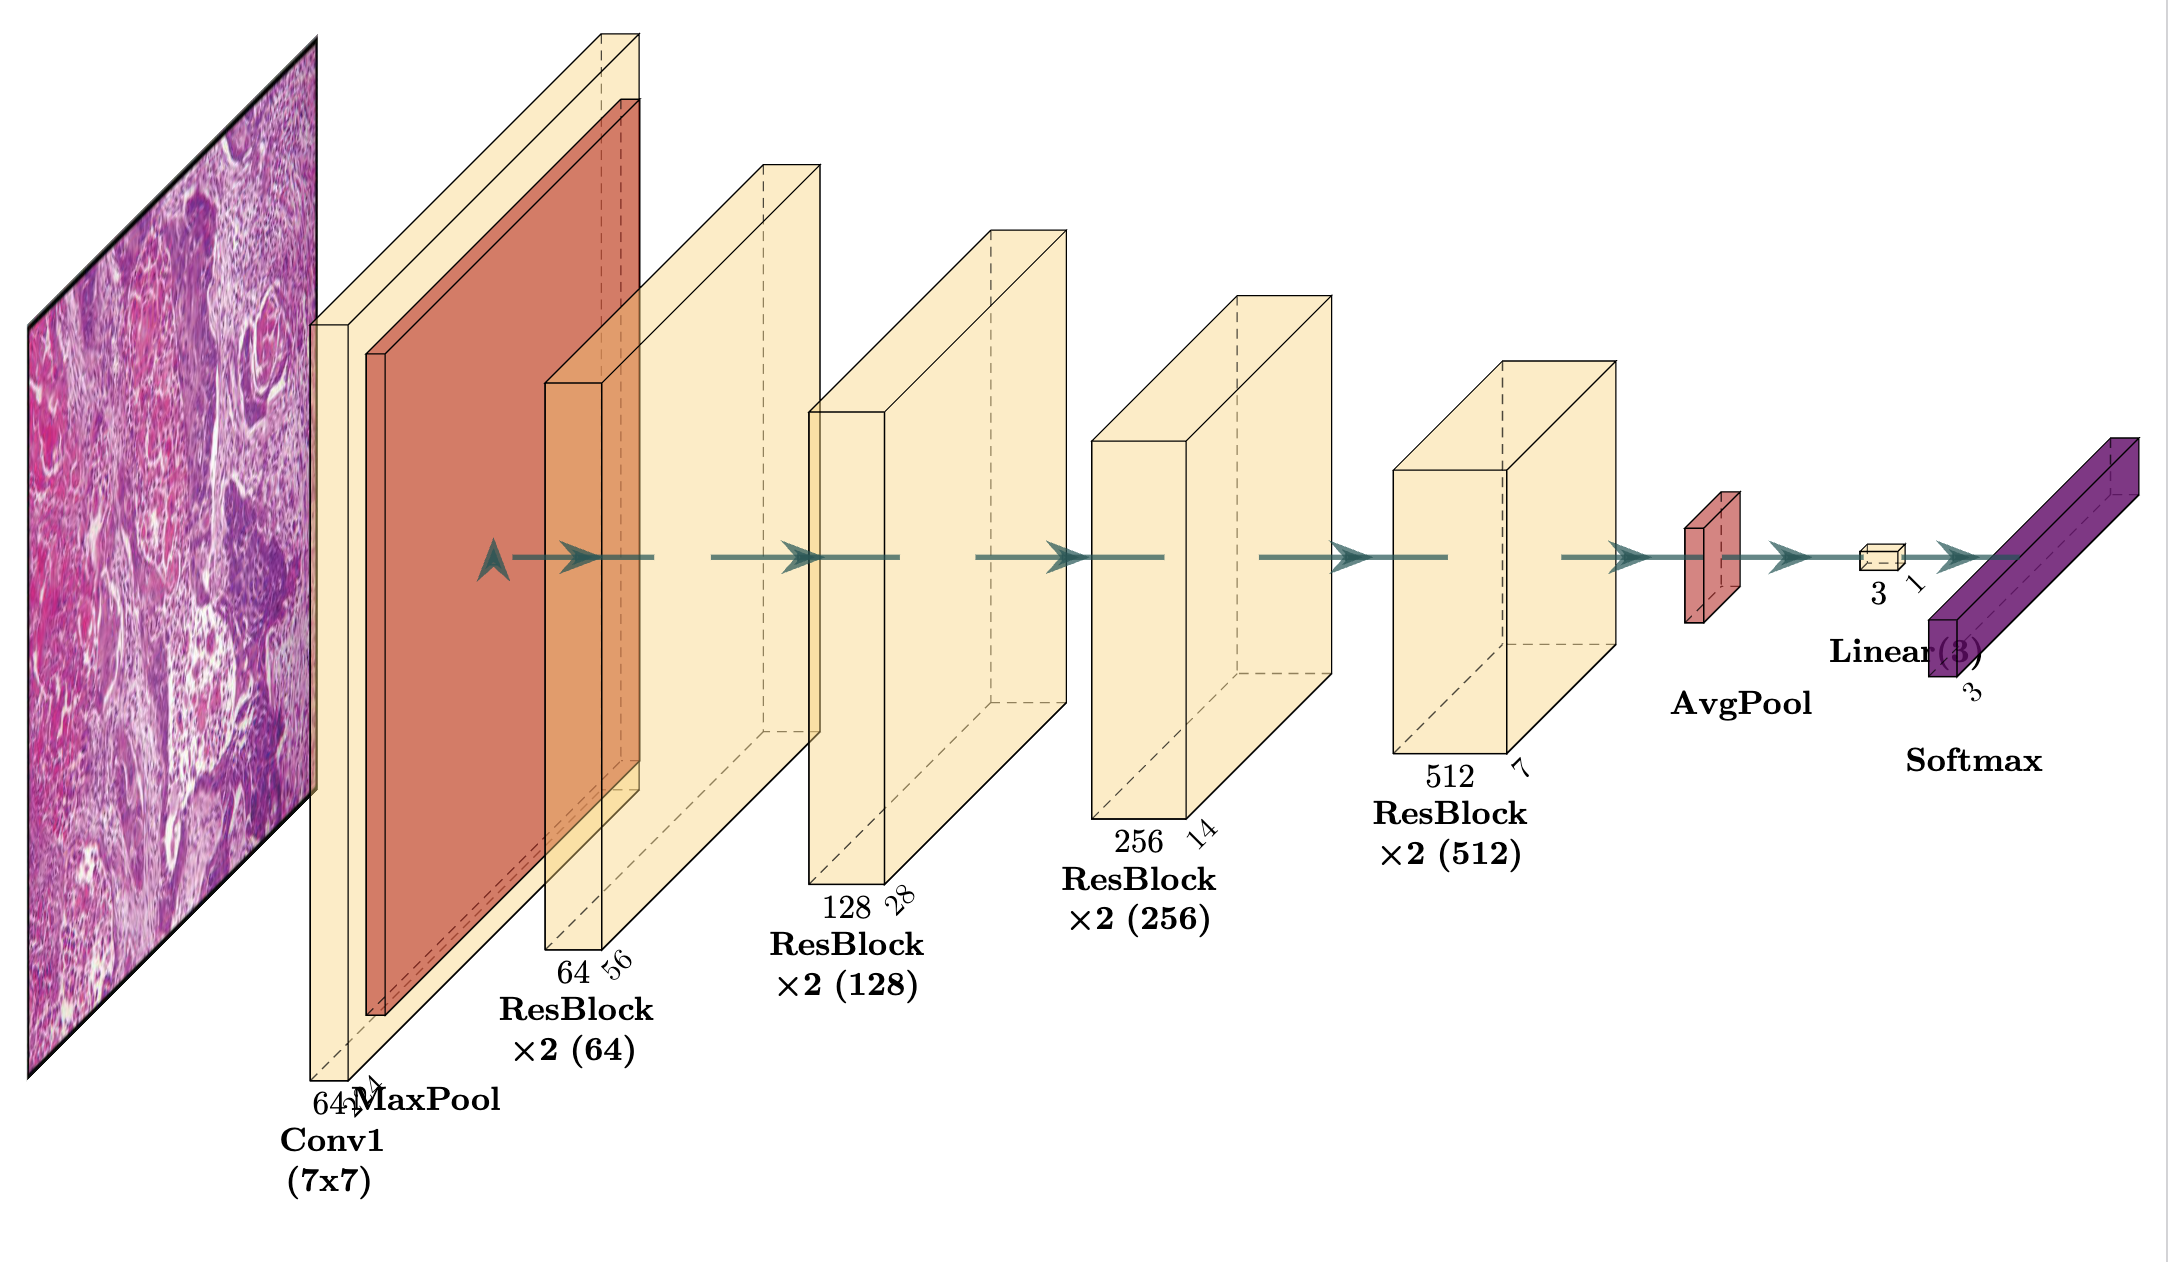
\includegraphics[width=0.48\textwidth]{resnetlung_architecture.png}
\caption{Arquitectura de la red \textit{ResNetLung}, con bloques residuales organizados en cuatro etapas y salida para tres clases.}
\label{fig:architecture}
\end{figure}


\subsection{Justificaci\'on de ResNet-18}
La elecci\'on de ResNet-18 se fundamenta en su equilibrio entre profundidad y eficiencia computacional. Estudios previos demuestran su eficacia en tareas m\'edicas similares. En \cite{xu2024resnet} se us\'o ResNet-18 para clasificaci\'on citol\'ogica respiratoria con buenos resultados. En \cite{wang2024pirads} se utiliz\'o exitosamente para clasificaci\'on de lesiones prost\'aticas.

\subsection{Entrenamiento}
El modelo se entrena usando Adam con tasa de aprendizaje de 0.001, funci\'on de p\'erdida CrossEntropy y 10 \'epocas. El entrenamiento se realiz\'o en un sistema Mac con soporte para MPS.

El modelo \textit{ResNetLung} fue entrenado durante 10 épocas utilizando el optimizador Adam con una tasa de aprendizaje inicial de $0.001$ y la función de pérdida \texttt{CrossEntropyLoss}. La Tabla~\ref{tab:epochacc} resume la evolución del desempeño del modelo a lo largo de las épocas. Se observa una disminución progresiva de la pérdida, desde $0.3668$ en la primera época hasta $0.1136$ en la última, acompañada de un incremento sostenido en la exactitud, alcanzando un valor final del $95.61\%$.

\begin{table}[ht]
\centering
\caption{Evolución del desempeño del modelo por época}
\begin{tabular}{|c|c|c|}
\hline
\textbf{Época} & \textbf{Loss} & \textbf{Accuracy} \\
\hline
1 & 0.3668 & 85.62\% \\
2 & 0.2530 & 89.48\% \\
3 & 0.1953 & 91.87\% \\
4 & 0.1860 & 92.57\% \\
5 & 0.1841 & 92.73\% \\
6 & 0.1511 & 94.03\% \\
7 & 0.1383 & 94.25\% \\
8 & 0.1284 & 94.93\% \\
9 & 0.1269 & 94.89\% \\
10 & \textbf{0.1136} & \textbf{95.61\%} \\
\hline
\end{tabular}
\label{tab:epochacc}
\end{table}

\section{Resultados y Análisis}

La Figura~\ref{fig:confmatrix} presenta la matriz de confusión obtenida tras evaluar el modelo sobre el conjunto de prueba. El clasificador muestra un rendimiento robusto en las tres clases analizadas: adenocarcinoma pulmonar (\texttt{lung\_aca}), tejido pulmonar sano (\texttt{lung\_n}) y carcinoma escamoso pulmonar (\texttt{lung\_scc}).

\begin{figure}[h]
\centering
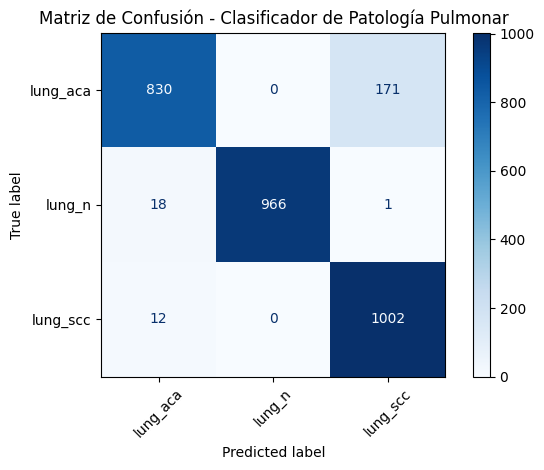
\includegraphics[width=0.45\textwidth]{confusion_matrix.png}
\caption{Matriz de confusión del modelo ResNetLung sobre el conjunto de prueba.}
\label{fig:confmatrix}
\end{figure}

Se destaca la clase \texttt{lung\_scc}, con $1002$ verdaderos positivos y únicamente $12$ falsos negativos. En contraste, la clase \texttt{lung\_aca} presentó una mayor tasa de error, con $830$ aciertos y $171$ instancias clasificadas erróneamente como \texttt{lung\_scc}. Esta confusión puede atribuirse a similitudes morfológicas entre los patrones celulares de ambas patologías, especialmente en cortes histológicos con estructuras glandulares mal diferenciadas.

En conjunto, los resultados sugieren que la arquitectura ResNet-18 implementada desde cero logra generalizar adecuadamente sobre el dominio de imágenes histopatológicas pulmonares. La progresión estable del entrenamiento y el alto rendimiento alcanzado sin señales de sobreajuste respaldan la idoneidad del modelo para esta tarea. El entrenamiento se ejecutó eficientemente en un entorno con soporte para \texttt{MPS} (Metal Performance Shaders), optimizado para equipos Apple.

\section{Conclusiones}

Los resultados presentados en este trabajo demuestran que una arquitectura residual de tipo ResNet-18, implementada desde cero, puede ser altamente efectiva para la clasificación multiclase de imágenes histopatológicas pulmonares. El modelo \textit{ResNetLung} logró una precisión final del 95.61\% tras solo 10 épocas de entrenamiento, mostrando una convergencia estable y progresiva, sin señales de sobreajuste.

La matriz de confusión evidenció un desempeño particularmente sólido en la clasificación de tejido sano y carcinoma escamoso, con tasas de verdaderos positivos superiores al 99\%. La mayor fuente de error se presentó al diferenciar adenocarcinoma de carcinoma escamoso, lo que sugiere que futuras mejoras podrían centrarse en técnicas de aumento de datos, ajuste fino o mecanismos de atención para capturar mejor las sutilezas morfológicas.

Gracias a su diseño modular, esta arquitectura puede escalar fácilmente a variantes más profundas como ResNet-34, incorporar técnicas de aprendizaje transferido o integrarse en pipelines clínicos asistidos por IA. En conjunto, \textit{ResNetLung} representa una solución computacional precisa, eficiente y extensible para apoyar el diagnóstico histopatológico del cáncer de pulmón.

\bibliographystyle{IEEEtran}
\begin{thebibliography}{1}

\bibitem{wang2024pirads}
W. Wang et al., ``PI-RADS 3 lesion classification based on ResNet18 in T2-weighted images,'' \emph{Frontiers in Oncology}, vol. 13, 2024.

\bibitem{xu2024resnet}
Y. Xu et al., ``Deep learning model based on an improved ResNet18 for on-site diagnosis of respiratory cytological samples,'' \emph{BMC Cancer}, vol. 24, no. 1, 2024.

\bibitem{he2016resnet}
K. He, X. Zhang, S. Ren, and J. Sun, ``Deep Residual Learning for Image Recognition,'' in \emph{Proc. of CVPR}, 2016.

\bibitem{kaggleLC25000}
Kaggle, ``Lung and Colon Cancer Histopathological Images,'' [Online]. Available: \url{https://www.kaggle.com/datasets/andrewmvd/lung-and-colon-cancer-histopathological-images}

\bibitem{paszke2019pytorch}
A. Paszke et al., ``PyTorch: An Imperative Style, High-Performance Deep Learning Library,'' in \emph{NeurIPS}, 2019.

\bibitem{resnetlunganon} ``LungCancer-ResNetClassifier,'' GitHub repository, 2025. [Online]. Available: \url{https://github.com/joelibaceta/LungCancer-ResNetClassifier}

\end{thebibliography}

\end{document}